% %%%%%%%%%%%%%%%%%%%%%%%%%%%%%%%%%%%%%%%%%%%%%%%%%%%%%%%%%%%%%%%%%%%%%%%%%%%%%%%%%%%%%%%%%%%%
% PROBLEM SET LATEX TEMPLATE FILE
% DEFINE DOCUMENT STYLE, LOAD PACKAGES
\documentclass[11pt,notitlepage]{article}\usepackage[]{graphicx}\usepackage[]{color}
%% maxwidth is the original width if it is less than linewidth
%% otherwise use linewidth (to make sure the graphics do not exceed the margin)
\makeatletter
\def\maxwidth{ %
  \ifdim\Gin@nat@width>\linewidth
    \linewidth
  \else
    \Gin@nat@width
  \fi
}
\makeatother

\definecolor{fgcolor}{rgb}{0.345, 0.345, 0.345}
\newcommand{\hlnum}[1]{\textcolor[rgb]{0.686,0.059,0.569}{#1}}%
\newcommand{\hlstr}[1]{\textcolor[rgb]{0.192,0.494,0.8}{#1}}%
\newcommand{\hlcom}[1]{\textcolor[rgb]{0.678,0.584,0.686}{\textit{#1}}}%
\newcommand{\hlopt}[1]{\textcolor[rgb]{0,0,0}{#1}}%
\newcommand{\hlstd}[1]{\textcolor[rgb]{0.345,0.345,0.345}{#1}}%
\newcommand{\hlkwa}[1]{\textcolor[rgb]{0.161,0.373,0.58}{\textbf{#1}}}%
\newcommand{\hlkwb}[1]{\textcolor[rgb]{0.69,0.353,0.396}{#1}}%
\newcommand{\hlkwc}[1]{\textcolor[rgb]{0.333,0.667,0.333}{#1}}%
\newcommand{\hlkwd}[1]{\textcolor[rgb]{0.737,0.353,0.396}{\textbf{#1}}}%
\let\hlipl\hlkwb

\usepackage{framed}
\makeatletter
\newenvironment{kframe}{%
 \def\at@end@of@kframe{}%
 \ifinner\ifhmode%
  \def\at@end@of@kframe{\end{minipage}}%
  \begin{minipage}{\columnwidth}%
 \fi\fi%
 \def\FrameCommand##1{\hskip\@totalleftmargin \hskip-\fboxsep
 \colorbox{shadecolor}{##1}\hskip-\fboxsep
     % There is no \\@totalrightmargin, so:
     \hskip-\linewidth \hskip-\@totalleftmargin \hskip\columnwidth}%
 \MakeFramed {\advance\hsize-\width
   \@totalleftmargin\z@ \linewidth\hsize
   \@setminipage}}%
 {\par\unskip\endMakeFramed%
 \at@end@of@kframe}
\makeatother

\definecolor{shadecolor}{rgb}{.97, .97, .97}
\definecolor{messagecolor}{rgb}{0, 0, 0}
\definecolor{warningcolor}{rgb}{1, 0, 1}
\definecolor{errorcolor}{rgb}{1, 0, 0}
\newenvironment{knitrout}{}{} % an empty environment to be redefined in TeX

\usepackage{alltt}    % ADD COMMENTS USING A PERCENT SIGN
\usepackage{amsfonts}
\usepackage{amsthm}
\usepackage{amsmath, booktabs}
\usepackage{mathtools}
\usepackage{amssymb}
\usepackage{subfig}
\usepackage{setspace}
\usepackage{fullpage}
\usepackage{verbatim}
\usepackage{graphicx}
\usepackage{tabularx}
\usepackage{longtable}
\usepackage{multicol}
\usepackage{multirow}
\setlength{\parindent}{0in}  	% uncomment to remove indent at start of paragraphs
\usepackage{pdflscape}
\usepackage[english]{babel}
\usepackage[pdftex]{hyperref}
\usepackage{natbib}
\usepackage{caption}
\usepackage{amsmath}
\usepackage{amsfonts}
\usepackage{graphics}
\usepackage{multirow}
\usepackage{graphics}
\usepackage{hyperref}
\usepackage{longtable}
\usepackage{latexsym}
\usepackage{rotating}
\usepackage{setspace}
\usepackage{layouts} 
\usepackage[titletoc]{appendix}
\DeclareGraphicsExtensions{.pdf,.jpg,.png}
\usepackage[margin=1in]{geometry}
\usepackage{enumerate}
\usepackage{float}

\newcolumntype{L}[1]{>{\raggedright\let\newline\\\arraybackslash\hspace{0pt}}m{#1}}
\newcolumntype{C}[1]{>{\centering\let\newline\\\arraybackslash\hspace{0pt}}m{#1}}
\newcolumntype{R}[1]{>{\raggedleft\let\newline\\\arraybackslash\hspace{0pt}}m{#1}}

\usepackage[T1]{fontenc}			

\usepackage{xcolor}
\usepackage[printwatermark]{xwatermark}





\title{Field Experiments: Design, Analysis and Interpretation \\
Solutions for Chapter 5 Exercises}
\author{Alan S. Gerber and Donald P. Green\footnote{Solutions prepared by Peter M. Aronow and revised by Alexander Coppock}}
\date{\vspace{-5ex}}


%%%%%%%%%%%%%%%%%%%%%%%%%%%%%%%%%%%%%%%%%%%%%%%%%%%%%%%%%%%%%%%%%%%%%%%%%%%%%%%%%%%%%%%%%%%%%
\IfFileExists{upquote.sty}{\usepackage{upquote}}{}
\begin{document}

\maketitle

\section*{Question 1}
Using the data in Table 5.2: [5 pts]
\begin{enumerate}[a)]
\item Estimate the following quantities: $E[d_i(1)]$, $E[Y_i(0)|d_i(1) = 0]$, $E[Y_i(0)| d_i(1) = 1]$,and $E[Y_i(1)|d_i(1)=1]$.\\
\begin{align*}
E[d_i(1)] &= \frac{395}{1445} = 0.273\\
E[(Y_i(0)|d_i(1) = 0)] &= 36.48\\
E[(Y_i(0)|d_i(1) = 1)] &= \frac{37.54 - (.727*36.48)}{0.273} = 40.36\\
E[(Y_i(1)|d_i(1) = 1)] &= 54.43
\end{align*}

\item Using these estimates and assuming that $E[Y_i(1)|d_i(1) = 0] = 0.5$, construct a figure that follows the format of Figure 5.1. Show the apparent proportion of Compliers, the ITT, and the CACE.

\begin{figure}[H]
    \centering
        \caption{Question 2 Figure}
    \subfloat[Treatment Group]{{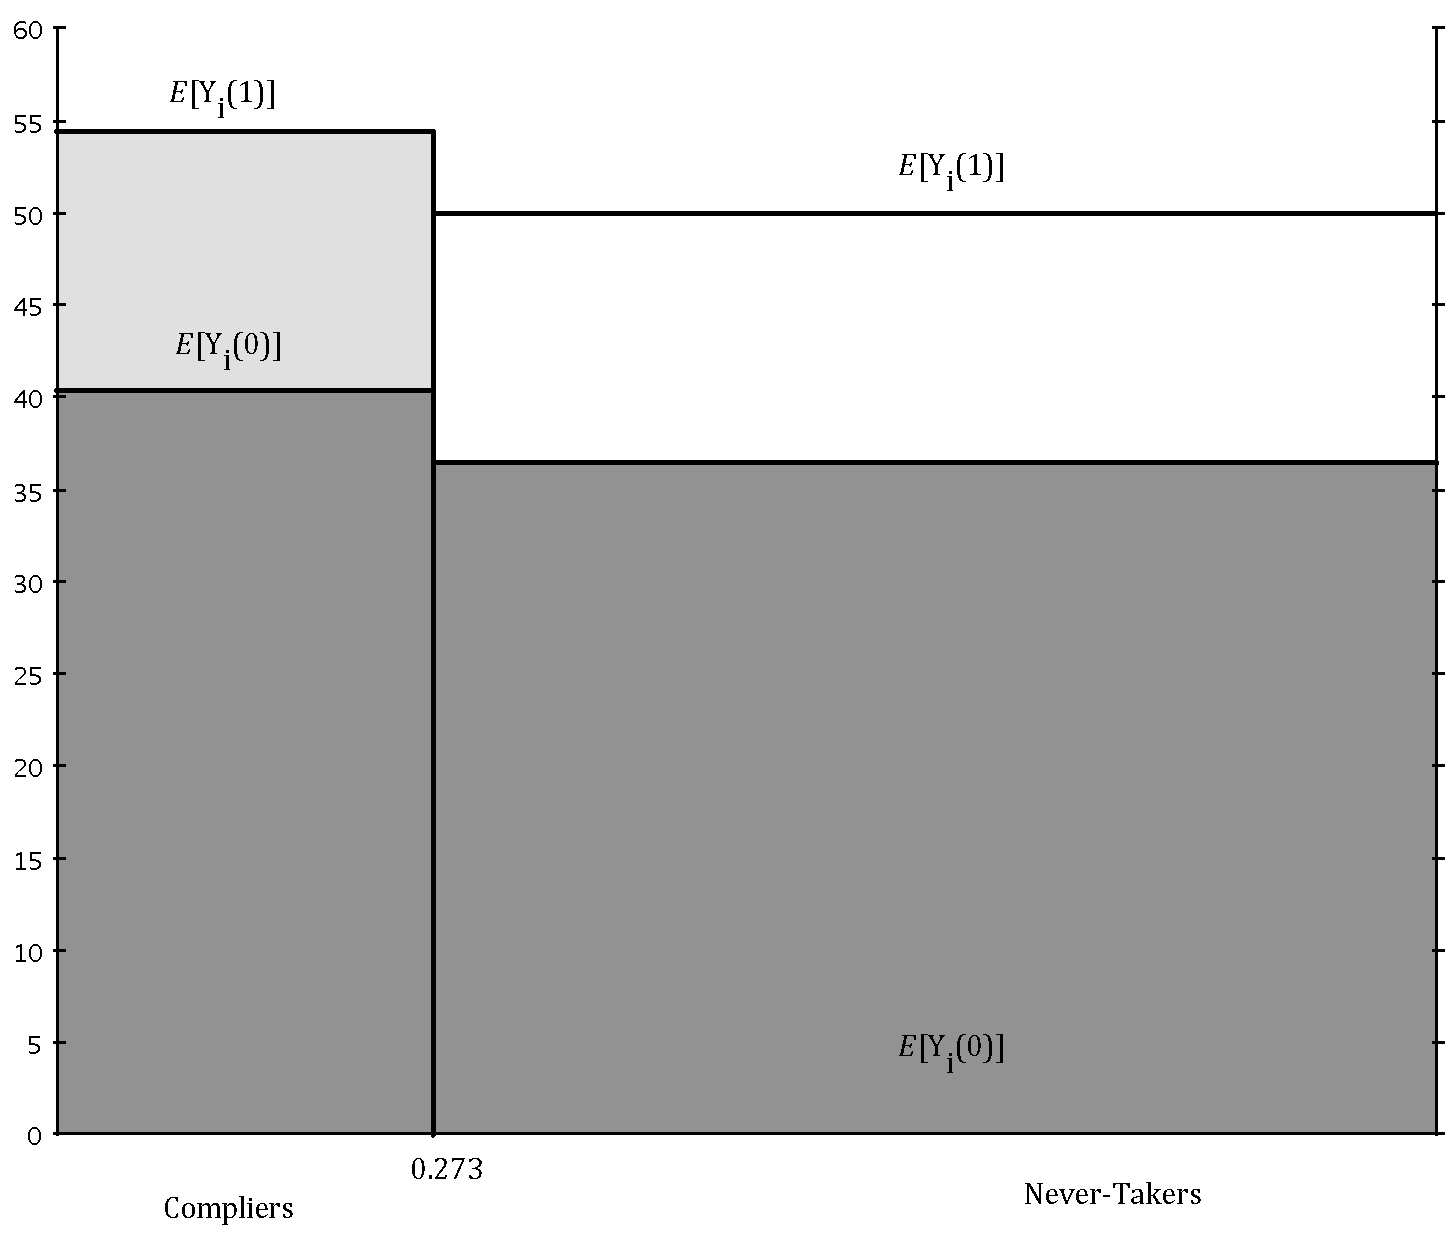
\includegraphics[width=7cm]{PS61btreatment.pdf} }}
    \qquad
    \subfloat[Control Group]{{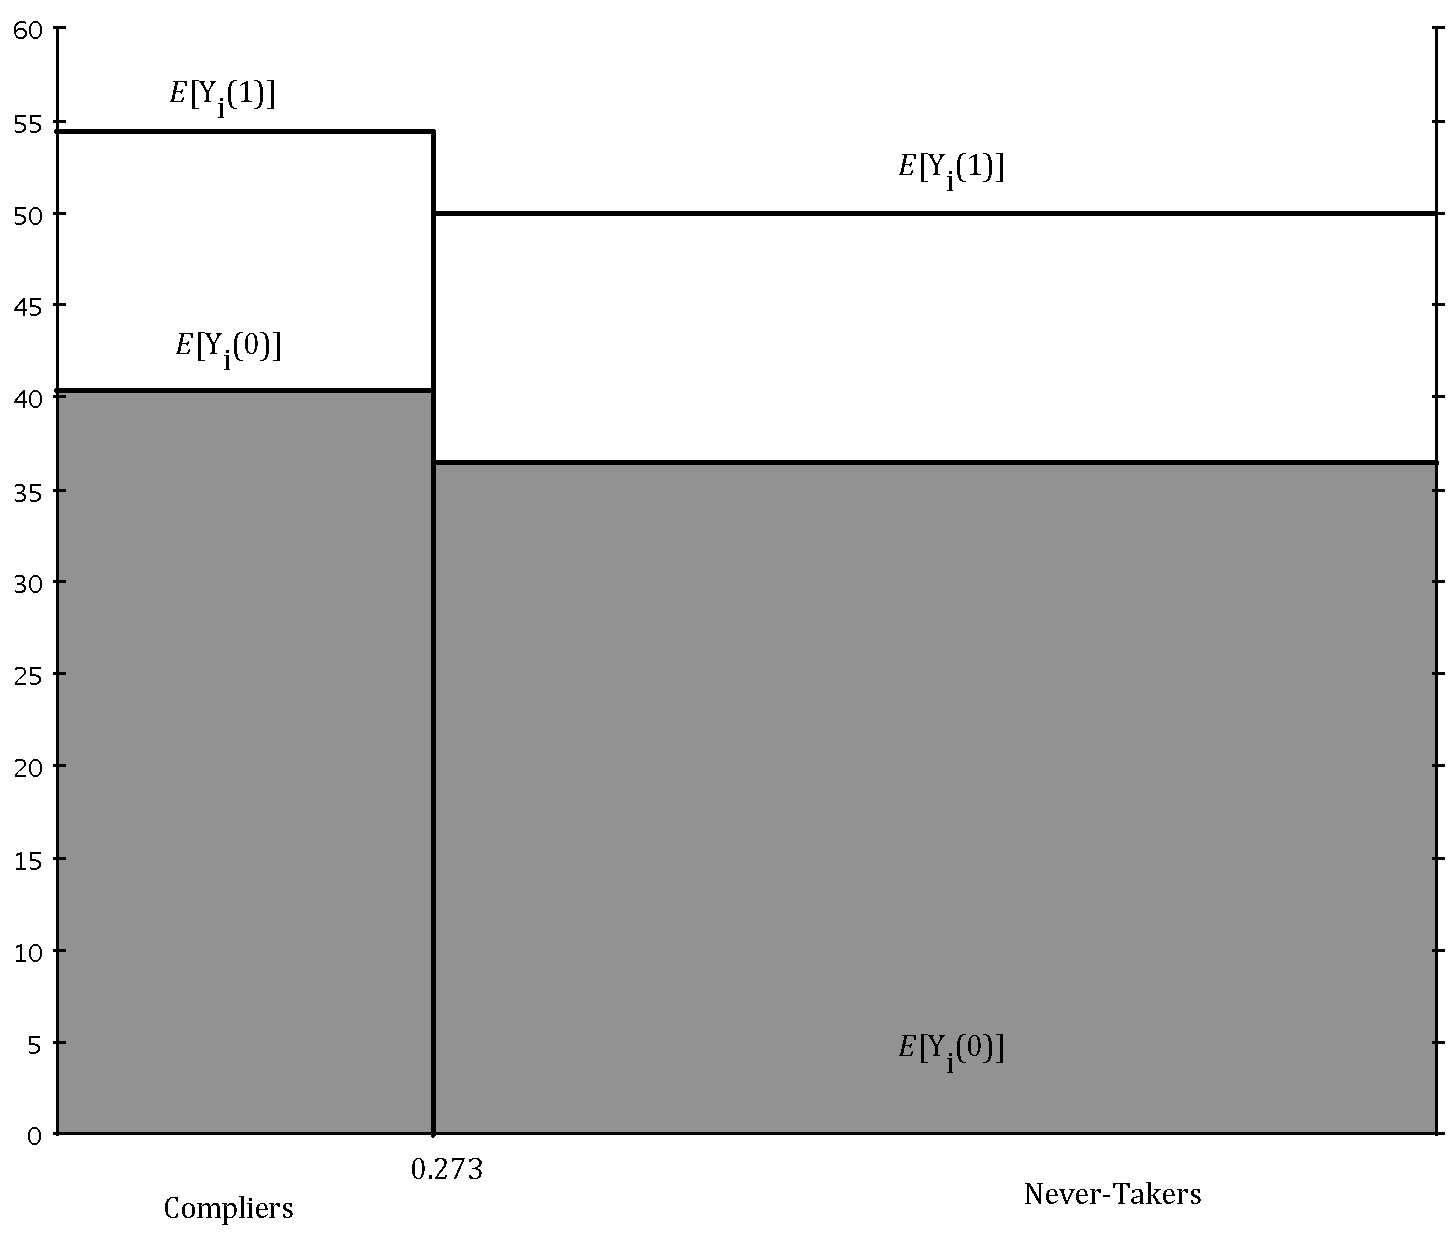
\includegraphics[width=7cm]{PS61bcontrol.pdf} }}
\end{figure}

\end{enumerate}


\section*{Question 2}

\begin{knitrout}
\definecolor{shadecolor}{rgb}{0.969, 0.969, 0.969}\color{fgcolor}\begin{kframe}
\begin{verbatim}





\end{verbatim}
\end{kframe}
\end{knitrout}



\section*{Question 3}
Explain whether each of the following statements is true or false for the case of one-sided noncompliance, assuming that an experiment satisfies non-interference and excludability. [8 pts.]
\begin{enumerate}[a)]
\item If the $ITT$ is negative, the $CACE$ must be negative.\\
Answer:\\
True. The $ITT$ can be written as $E[D(1)]*CACE$. If this quantity is negative, then since $E[D(1)]$ must be non-negative, the $CACE$ must be negative.  
\item The smaller the $ITT_D$, the larger the $CACE$.\\
Answer:\\
False. There is no necessary relationship between the $ITT_D$, the proportion of the subjects that are compliers, and the CACE, the average response of the compliers to the treatment. This confusion sometimes arises due to the algebra of calculating the CACE from the $ITT$ and $ITT_D$. Because the $ITT$ can be written as $ITT_D*CACE$, the $CACE$ can be calculated by $ITT/ITT_D$. From this ratio it might appear that when the $ITT_D$ is smaller we are dividing the ITT by a smaller number, leading to a larger CACE. However, the $ITT$ is a function of the $ITT_D$: the $ITT_D$ is in both the numerator (multiplied by the $CACE$) and the denominator.
\item One cannot identify the CACE if no one in the experiment receives the treatment.\\
Answer:\\
True. If no one receives the treatment, it is impossible to estimate the effect of the treatment. Algebraically, the ITT estimate is divided by zero, leading to an undefined CACE estimate. 
\end{enumerate}

\section*{Question 4}
\begin{knitrout}
\definecolor{shadecolor}{rgb}{0.969, 0.969, 0.969}\color{fgcolor}\begin{kframe}
\begin{verbatim}





\end{verbatim}
\end{kframe}
\end{knitrout}

\section*{Question 5}
Critically evaluate the following statement: ``If you are conducting an experiment that encounters one-sided noncompliance, you will never know which of your subjects are Compliers and which of your subjects are Never-Takers.'' [5 pts.]\\
Answer:\\
Subjects are assigned to treatment or control. For those subjects assigned to the control group, all subjects are untreated so there is no way to distinguish among them. For those subject assigned to the treatment group, the Compliers are treated and the Never-Takers are not. This is observable, and so you can tell which subjects are of each type for those assigned to the treatment group. Using the subjects assigned to the treatment group, you can contrast the compliers and never-takers based on pretreatment variables.  However, as suggested by the statement, there is a limit to what you can know about individual subjects assigned to the control group. Since both types remain untreated in the control group, you cannot partition the entire subject pool into compliers and never takers.

\section*{Question 6}
\begin{knitrout}
\definecolor{shadecolor}{rgb}{0.969, 0.969, 0.969}\color{fgcolor}\begin{kframe}
\begin{verbatim}





\end{verbatim}
\end{kframe}
\end{knitrout}


\section*{Question 7}
Make up a schedule of potential outcomes that would generate Figure 5.2, which illustrates the consequences of an exclusion restriction violation. Hint: you will need to allow for potential outcomes that respond to both $d$ and $z$. [5 pts.]\\
Answer:\\
Figure 5.2 illustrates a situation in which the potential outcome when untreated among the non-compliers depends on whether the subject is in the treatment versus control group. Note that this is just an example of an exclusion restriction violation, in this case limited to one of the average potential outcomes (untreated non-compliers). Other patterns of ER violations are possible as well.
The 6 quantities needed to construct a figure similar to figure 5.2 are: 
\begin{enumerate}
\item $E[D_i(1)]$
\item $E[(Y(0)|D_i(1) = 0), Z_i = 0]$
\item $E[(Y(0)|D_i(1) = 0), Z_i = 1]$
\item $E[(Y(1)|D_i(1) = 0)]$
\item $E[(Y(0)|D_i(1) = 1)]$
\item $E[(Y(1)|D_i(1) = 1)]$
\end{enumerate}
Further, $E[(Y(0)|D_i(1) = 0), Z_i = 0]$ and $E[(Y(0)|D_i(1) = 0), Z_i = 1]$ must be different -- this is the crucial violation of the exclustion restriction. Suppose the subject pool is comprised of only two type subjects. 25 percent are of type 1 and the remainder are of type 2.

\begin{table}[H]
  \centering
  \caption{Question 7 Table}
    \begin{tabular}{lllll}
    \toprule
    Subject  & $Y(D=1)$ & $Y(D=0, Z=0)$ & $Y(D=0, Z=1)$ & $D(1)$ \\
    \midrule
    Type 1 & 10    & 5     & 5     & 1 \\
    Type 2 & 8     & 4     & 6     & 0 \\
    \bottomrule
    \end{tabular}%
  \label{tab:addlabel}%
\end{table}%

\section*{Question 8}
\begin{knitrout}
\definecolor{shadecolor}{rgb}{0.969, 0.969, 0.969}\color{fgcolor}\begin{kframe}
\begin{verbatim}





\end{verbatim}
\end{kframe}
\end{knitrout}


\section*{Question 9}
One way to detect heterogeneous treatment effects across subgroups is to employ a design that randomly manipulates the level of compliance. One such study was conducted in Michigan in 2002.\footnote{Gerber and Green 2005.} Subjects were randomly allocated to three experimental groups. The first treatment group was targeted for a phone call that encouraged subjects to vote in the upcoming November election. The second treatment group was targeted for the same call using the same script on the same day, but more attempts were made to reach subjects. No attempts were made to contact the control group. The table below shows the contact rates and voting rates for each of the three assigned groups. [10 pts.]

\begin{table}[H]
  \centering
  \caption{Question 9 Table}
    \begin{tabular}{rrR{3.5cm}R{3.5cm}}
    \toprule
          & Control  & Treatment group \#1 (minimal effort)  & Treatment group \#2 (maximal effort)  \\
    \midrule
    Percent reached by callers  & 0     & 29.97 & 47.31 \\
    Percent voting  & 55.89 & 55.91 & 56.53 \\
    N     & 317182 & 7500  & 7500 \\
    \bottomrule
    \end{tabular}%
  \label{tab:addlabel}%
\end{table}%

\begin{enumerate}[a)]
\item Define two types of Compliers: those who respond when called with minimal (or maximal) effort and those who respond only when called with maximal effort. Write down a model expressing the expected voting rate among those assigned to the control group as a weighted average of potential outcomes among Minimal Compliers, Maximal Compliers, and Never-Takers. Do the same for the expected rate of voting among those assigned to each of the treatment groups.\\
Answer:\\
Let $Z_i = 0$ (no call), $1$ (minimal effort), or $2$ (maximal effort). $Y_i(Z_i) =1$ if subject $i$ votes, $0$ otherwise. Assuming monotonicity as outlined in the problem description, there are three types ($D_i(0)=0$ for all types): 
\begin{itemize}
\item $D_i(1) = D_i(2) = 0$   [Never-Takers]
\item $D_i(2) = 1, D_i(1)=1$	[Easy to reach subjects, or Minimal Effort Compliers]
\item $D_i(2) = 1, D_i(1) = 0$	[Hard to reach subjects, or Maximal Effort Compliers]
\end{itemize}

\begin{align*}
\text{Expected Vote rate in Control (EV, Control)} &= \\
&E(Y(0)|\text{ never taker})*Pr(\text{never taker}) + \\
&E(Y(0)|\text{ easy to reach})*Pr(\text{easy to reach}) + \\
&E(Y(0)|\text{ hard to reach})*Pr(\text{hard to reach})
\end{align*}

\begin{align*}
\text{Expected Vote rate in minimal effort (EV, minimal)} &= \\
&E(Y(0)|\text{ never taker})*Pr(\text{never taker}) + \\
&E(Y(1)|\text{ easy to reach})*Pr(\text{easy to reach}) + \\
&E(Y(0)|\text{ hard to reach})*Pr(\text{hard to reach})
\end{align*}

\begin{align*}
\text{Expected Vote rate in maximal effort (EV, maximal)} &= \\
&E(Y(0)|\text{ never taker})*Pr(\text{never taker}) + \\
&E(Y(1)|\text{ easy to reach})*Pr(\text{easy to reach}) + \\
&E(Y(1)|\text{ hard to reach})*Pr(\text{hard to reach})
\end{align*}


\item Show that the CACE for each of the treatments can be identified based on the design of this experiment.

\begin{align*}
\text{(EV, minimal - EV,control)} &= \\
&E(Y(1)|\text{ easy to reach})*Pr(\text{easy to reach}) - \\
&E(Y(0)|\text{ easy to reach})*Pr(\text{easy to reach}) \\
&= E(Y(1) -(Y(0)|\text{ easy to reach})*Pr(\text{easy to reach}) \\
&= (\text{ATE}|\text{ easy to reach})*Pr(\text{easy to reach}). \\
\text{ATE|\text{ easy to reach}} &= \frac{\text{(EV, minimal - EV,control)}}{Pr(\text{easy to reach})}
\end{align*}

Similarly, 
\begin{align*}
\text{(EV, maximal - EV,minimal)} &= \\
&E(Y(1)|\text{ hard to reach})*Pr(\text{hard to reach}) - \\
&E(Y(0)|\text{ hard to reach})*Pr(\text{hard to reach}) \\
&= E(Y(1) -(Y(0)|\text{ hard to reach})*Pr(\text{hard to reach}) \\
&= (\text{ATE}|\text{ hard to reach})*Pr(\text{hard to reach}). \\
\text{ATE|\text{ hard to reach}} &= \frac{\text{(EV, maximal - EV,minimal)}}{Pr(\text{hard to reach})}
\end{align*}

To estimate the numerators, which involve EV for the subject pool when untreated, given the minimal treatment or maximal treatment, use the average of the randomly assigned groups, which are unbiased estimators of the respective quantities.
To obtain unbiased estimates of the subject pool proportions for the three types, the proportion that complies in the minimal treatment group is an unbiased estimate of the proportion of easy to reach, and the proportion that complies in the maximal effort group is an estimate of the combined proportion of easy and hard to reach. Subtract the estimated proportion that is easy to reach to obtain the proportion that is hard to reach.


\item Estimate the share of the subject pool that Maximal Compliers comprise. Estimate the share of the subject pool that Minimal Compliers comprise.\\
Answer:\\
The share of compliers in the minimal treatment group provides an estimate of the share of easy to reach: 29.97\% \\
The share of compliers in the maximal treatment group provides an estimate of the share of easy to reach plus the share of hard to reach, which equals 47.31. Subtracting the estimated share of the easy to reach, 29.97\%, produces an estimate of the share of hard to reach, 47.31 - 29.97 = 17.34\%. 

\item Estimate the average treatment effect among each type of Complier, and interpret the results.
Answer:\\
The CACE for the easy to reach: $\frac{0.5591 - 0.5589}{0.2997} = 0.0007$ \\ 
The CACE for the hard to reach: $\frac{0.5653 - 0.5591}{0.1734} = 0.0358$ \\
The treatment effect estimate for the hard to reach is larger than the estimated effect for the easy to reach, although further calculations are needed to determine whether the difference in CACEs is greater than one would expect from random sampling variability.

\end{enumerate}

\section*{Question 10}
\begin{knitrout}
\definecolor{shadecolor}{rgb}{0.969, 0.969, 0.969}\color{fgcolor}\begin{kframe}
\begin{verbatim}





\end{verbatim}
\end{kframe}
\end{knitrout}


\section*{Question 11}
Nickerson describes a voter mobilization experiment in which subjects were randomly assigned to one of three conditions: a baseline group (no contact was attempted), a treatment group (canvassers attempted to deliver an encouragement to vote), and a placebo group (canvassers attempted to deliver an encouragement to recycle).\footnote{Nickerson 2005, 2008.} Based on the results presented below, calculate the following: [10 pts.]
% Table generated by Excel2LaTeX from sheet 'Sheet1'
\begin{table}[H]
  \centering
  \caption{Question 11 Table}
    \begin{tabular}{rrrr}
    \toprule
    Treatment assignment  & Treated?  & N     & Turnout  \\
    \midrule
    \multicolumn{1}{c}{Baseline}  & No    & 2572  & 0.3122 \\
    \multicolumn{1}{c}{\multirow{2}[0]{*}{Treatment }} & Yes   & 486   & 0.3909 \\
    \multicolumn{1}{c}{} & No    & 2086  & 0.3274 \\
    \multicolumn{1}{c}{\multirow{2}[0]{*}{Placebo }} & Yes   & 470   & 0.2979 \\
    \multicolumn{1}{c}{} & No    & 2109  & 0.3215 \\
    \bottomrule
    \end{tabular}%
  \label{tab:addlabel}%
\end{table}%

\begin{enumerate}[a)]
\item Estimate the proportion of Compliers based on subjects' responses to the treatment.
Estimate the proportion of Compliers based on subjects' responses to the placebo. Assuming that the individuals are assigned randomly to the treatment and placebo groups, are these rates of compliance consistent with the null hypothesis that both groups have the same proportion of Compliers? \\

\begin{knitrout}
\definecolor{shadecolor}{rgb}{0.969, 0.969, 0.969}\color{fgcolor}\begin{kframe}
\begin{alltt}
\hlstd{Z} \hlkwb{<-} \hlkwd{c}\hlstd{(}\hlkwd{rep}\hlstd{(}\hlstr{"baseline"}\hlstd{,} \hlnum{2572}\hlstd{),} \hlkwd{rep}\hlstd{(}\hlstr{"treatment"}\hlstd{,} \hlnum{486}\hlopt{+}\hlnum{2086}\hlstd{),} \hlkwd{rep}\hlstd{(}\hlstr{"placebo"}\hlstd{,} \hlnum{470}\hlopt{+}\hlnum{2109}\hlstd{))}
\hlstd{D} \hlkwb{<-} \hlkwd{c}\hlstd{(}\hlkwd{rep}\hlstd{(}\hlnum{0}\hlstd{,} \hlnum{2572}\hlstd{),} \hlkwd{rep}\hlstd{(}\hlnum{1}\hlstd{,} \hlnum{486}\hlstd{),} \hlkwd{rep}\hlstd{(}\hlnum{0}\hlstd{,}\hlnum{2086}\hlstd{),} \hlkwd{rep}\hlstd{(}\hlnum{1}\hlstd{,} \hlnum{470}\hlstd{),} \hlkwd{rep}\hlstd{(}\hlnum{0}\hlstd{,}\hlnum{2109}\hlstd{))}
\hlstd{Y} \hlkwb{<-} \hlkwd{c}\hlstd{(}\hlkwd{rep}\hlstd{(}\hlnum{1}\hlstd{,} \hlkwd{round}\hlstd{(}\hlnum{2572}\hlopt{*}\hlnum{0.3122}\hlstd{)),} \hlkwd{rep}\hlstd{(}\hlnum{0}\hlstd{,}\hlkwd{round}\hlstd{(}\hlnum{2572}\hlopt{*}\hlstd{(}\hlnum{1}\hlopt{-}\hlnum{0.3122}\hlstd{))),}
       \hlkwd{rep}\hlstd{(}\hlnum{1}\hlstd{,} \hlkwd{round}\hlstd{(}\hlnum{486}\hlopt{*}\hlnum{0.3909}\hlstd{)),} \hlkwd{rep}\hlstd{(}\hlnum{0}\hlstd{,}\hlkwd{round}\hlstd{(}\hlnum{486}\hlopt{*}\hlstd{(}\hlnum{1}\hlopt{-}\hlnum{0.3909}\hlstd{))),}
       \hlkwd{rep}\hlstd{(}\hlnum{1}\hlstd{,} \hlkwd{round}\hlstd{(}\hlnum{2086}\hlopt{*}\hlnum{0.3274}\hlstd{)),} \hlkwd{rep}\hlstd{(}\hlnum{0}\hlstd{,}\hlkwd{round}\hlstd{(}\hlnum{2086}\hlopt{*}\hlstd{(}\hlnum{1}\hlopt{-}\hlnum{0.3274}\hlstd{))),}
       \hlkwd{rep}\hlstd{(}\hlnum{1}\hlstd{,} \hlkwd{round}\hlstd{(}\hlnum{470}\hlopt{*}\hlnum{0.2979}\hlstd{)),} \hlkwd{rep}\hlstd{(}\hlnum{0}\hlstd{,}\hlkwd{round}\hlstd{(}\hlnum{470}\hlopt{*}\hlstd{(}\hlnum{1}\hlopt{-}\hlnum{0.2979}\hlstd{))),}
       \hlkwd{rep}\hlstd{(}\hlnum{1}\hlstd{,} \hlkwd{round}\hlstd{(}\hlnum{2109}\hlopt{*}\hlnum{0.3215}\hlstd{)),} \hlkwd{rep}\hlstd{(}\hlnum{0}\hlstd{,}\hlkwd{round}\hlstd{(}\hlnum{2109}\hlopt{*}\hlstd{(}\hlnum{1}\hlopt{-}\hlnum{0.3215}\hlstd{))))}
\hlstd{pr.c.treatment} \hlkwb{<-} \hlkwd{mean}\hlstd{(D[Z}\hlopt{==}\hlstr{"treatment"}\hlstd{])}
\hlstd{pr.c.treatment}
\end{alltt}
\begin{verbatim}
## [1] 0.189
\end{verbatim}
\begin{alltt}
\hlstd{pr.c.placebo} \hlkwb{<-} \hlkwd{mean}\hlstd{(D[Z}\hlopt{==}\hlstr{"placebo"}\hlstd{])}
\hlstd{pr.c.placebo}
\end{alltt}
\begin{verbatim}
## [1] 0.1822
\end{verbatim}
\end{kframe}
\end{knitrout}

The estimated proportion of compliers in the vote encouragement group is 0.189. The estimated proportion in the placebo group is 0.182. The difference between these rates is fairly small and not statistically significant. These rates of compliance are consistent with the null hypothesis that both groups have the same proportion of Compliers.

\item Do the data suggest that Never-Takers in the treatment and placebo groups have the same rate of turnout? Is this comparison informative?\\
\begin{knitrout}
\definecolor{shadecolor}{rgb}{0.969, 0.969, 0.969}\color{fgcolor}\begin{kframe}
\begin{alltt}
\hlstd{rate.nt.treatment} \hlkwb{<-} \hlkwd{mean}\hlstd{(Y[Z}\hlopt{==}\hlstr{"treatment"} \hlopt{&} \hlstd{D}\hlopt{==}\hlnum{0}\hlstd{])}
\hlstd{rate.nt.placebo} \hlkwb{<-} \hlkwd{mean}\hlstd{(Y[Z}\hlopt{==}\hlstr{"placebo"} \hlopt{&} \hlstd{D}\hlopt{==}\hlnum{0}\hlstd{])}
\hlstd{rate.nt.treatment}
\end{alltt}
\begin{verbatim}
## [1] 0.3274
\end{verbatim}
\begin{alltt}
\hlstd{rate.nt.placebo}
\end{alltt}
\begin{verbatim}
## [1] 0.3215
\end{verbatim}
\end{kframe}
\end{knitrout}
Yes, the turnout rate among the encouragement never takers is 32.7\% versus 32.2\% for the placebo group. If $D_i(1)$ is the same for all subjects whether the $Z=1$ means that they are assigned to the placebo or the encouragement, and the subjects are randomly assigned to each group, then the groups of untreated placebo and encouragement subjects are formed by random assignment from the same pool of subjects (the non-compliers). A prediction that follows from this claim is that placebo and the encouragement groups have the same expected average potential outcomes when untreated. If the observed difference in average potential outcomes when untreated is too large, we may reject the maintained hypothesis that the group is formed by random draws from a common pool of subjects. One implication of this is that perhaps the pattern of subject compliance is not the same for the two treatments.

\item Estimate the CACE of receiving the placebo. Is this estimate consistent with the substantive assumption that the placebo has no effect on turnout?\\
\begin{knitrout}
\definecolor{shadecolor}{rgb}{0.969, 0.969, 0.969}\color{fgcolor}\begin{kframe}
\begin{alltt}
\hlstd{itt.placebo} \hlkwb{<-} \hlkwd{mean}\hlstd{(Y[Z}\hlopt{==}\hlstr{"placebo"}\hlstd{])} \hlopt{-} \hlkwd{mean}\hlstd{(Y[Z}\hlopt{==}\hlstr{"baseline"}\hlstd{])}
\hlstd{cace.placebo} \hlkwb{<-} \hlstd{itt.placebo}\hlopt{/}\hlstd{pr.c.placebo}
\end{alltt}
\end{kframe}
\end{knitrout}

The CACE is 0.027. The placebo has an unexpectedly positive effect on turnout (although further analysis shows that the effect is not larger than one would expect due to random sampling variability). The fact that the placebo group has higher turnout than the control group makes the GOTV vs. placebo comparison more conservative.

\item Estimate the CACE of receiving the treatment using two different methods. First, use the conventional method of dividing the $ITT$ by the $ITT_D$. Second, compare turnout rates among Compliers in both the treatment and placebo groups. Interpret the results. \\
\begin{knitrout}
\definecolor{shadecolor}{rgb}{0.969, 0.969, 0.969}\color{fgcolor}\begin{kframe}
\begin{alltt}
\hlcom{## Method 1}
\hlstd{itt.treatment} \hlkwb{<-} \hlkwd{mean}\hlstd{(Y[Z}\hlopt{==}\hlstr{"treatment"}\hlstd{])} \hlopt{-} \hlkwd{mean}\hlstd{(Y[Z}\hlopt{==}\hlstr{"baseline"}\hlstd{])}
\hlstd{cace.treatment1} \hlkwb{<-} \hlstd{itt.treatment}\hlopt{/}\hlstd{pr.c.treatment}
\hlstd{cace.treatment1}
\end{alltt}
\begin{verbatim}
## [1] 0.1440329
\end{verbatim}
\begin{alltt}
\hlcom{## Method 2}
\hlstd{cace.treatment2} \hlkwb{<-} \hlkwd{mean}\hlstd{(Y[Z}\hlopt{==}\hlstr{"treatment"} \hlopt{&} \hlstd{D}\hlopt{==}\hlnum{1}\hlstd{])} \hlopt{-} \hlkwd{mean}\hlstd{(Y[Z}\hlopt{==}\hlstr{"placebo"} \hlopt{&} \hlstd{D}\hlopt{==}\hlnum{1}\hlstd{])}
\hlstd{cace.treatment2}
\end{alltt}
\begin{verbatim}
## [1] 0.09307416
\end{verbatim}
\end{kframe}
\end{knitrout}

Using the ITT and the compliance rate, the estimated average treatment effect for the compliers is a 14.4 percentage point increase in turnout. Comparing the compliers when treated and when untreated (assuming compliance with the placebo isolates the same group of subjects as compliance with the encouragement and the placebo has no effect of Y(0) for compliers), the estimated CACE is 9.3 percentage points. \\

The two methods arrive at similar estimates of the CACE. Because Method 1 involves a ratio estimator, it is biased but consistent.  Method 2 is both unbiased and consistent.  As noted above, the (chance) higher turnout in the placebo group makes Method 2 generate conservative estimates of the CACE in this case.
\end{enumerate}

\section*{Question 12}
\begin{knitrout}
\definecolor{shadecolor}{rgb}{0.969, 0.969, 0.969}\color{fgcolor}\begin{kframe}
\begin{verbatim}





\end{verbatim}
\end{kframe}
\end{knitrout}





\end{document}

